\documentclass[12pt,a4paper]{article}
\pdfoutput=1
 
%%
%% This huge block of usepackages does a lot of things.
%% It makes the text pritty on screens and ensures that you can use some common
%% tools.
%%
 
\usepackage[utf8]{inputenc}
\usepackage[T1]{fontenc}
% change language to whatever you write in
\usepackage[english]{babel}
\usepackage{amsmath}
\usepackage{lmodern}
\usepackage{listings}
\usepackage{units}
\usepackage{icomma}
\usepackage{color}
\usepackage{graphicx}
\usepackage{multicol,caption}
\usepackage{bbm}
\usepackage{hyperref}
\usepackage{xfrac}
\newcommand{\N}{\ensuremath{\mathbbm{N}}}
\newcommand{\Z}{\ensuremath{\mathbbm{Z}}}
\newcommand{\Q}{\ensuremath{\mathbbm{Q}}}
\newcommand{\R}{\ensuremath{\mathbbm{R}}}
\newcommand{\C}{\ensuremath{\mathbbm{C}}}
\newcommand{\rd}{\ensuremath{\mathrm{d}}}
\newcommand{\id}{\ensuremath{\,\rd}}

\definecolor{dkgreen}{rgb}{0,0.6,0}
\definecolor{gray}{rgb}{0.5,0.5,0.5}
\definecolor{mauve}{rgb}{0.58,0,0.82}

%Code color coding
\lstset{frame=tb,
  language=Matlab,
  aboveskip=3mm,
  belowskip=3mm,
  showstringspaces=false,
  columns=flexible,
  basicstyle={\small\ttfamily},
  numbers=none,
  numberstyle=\tiny\color{gray},
  keywordstyle=\color{blue},
  commentstyle=\color{dkgreen},
  stringstyle=\color{mauve},
  breaklines=true,
  breakatwhitespace=true,
  tabsize=3
}
 
%  if you want a page header/footer, use this!
% \usepackage{fancyhdr}
% \pagestyle{fancy}
% \lhead{Left in the header}
% \rhead{Right in the header: \today}
 
% This creates a nice figure environment that puts the image where you use it,
% and not where LaTeX wants it to be.
\newenvironment{Figure}
  {\par\medskip\noindent\minipage{\linewidth}}
  {\endminipage\par\medskip}
 
% neat horisontal line
\newcommand{\HRule}{\rule{\linewidth}{0.5mm}}
 
\begin{document}
 
\title{The title}
\author{The author}
\date{\today}
 
%%
%% Use one of these title methods
%%
% \maketitle % simple latex title
\begin{titlepage}
\begin{center}
 
% Pre-title
\textsc{\Large TNM034 2014}\\[0.5cm]
 
% Title
\HRule \\[0.4cm]
{ \huge \bfseries An Automated Pipeline for Extracting and Decoding QR-codes from Arbitrary Images \\[0.4cm] }
 
\HRule \\[1.5cm]
 
% Author and supervisor
\begin{minipage}{0.4\textwidth}
\begin{flushleft} \large
% Author
John Holl\'en\\
\emph{johho982@student.liu.se}
\end{flushleft}
\end{minipage}
\begin{minipage}{0.4\textwidth}
\begin{flushright} \large
Simon Bergstr\"om\\
\emph{simbe109@student.liu.se}
\end{flushright}
\end{minipage}
 
\vfill
 
% Bottom of the page
{\large \today}
 
\end{center}
\end{titlepage} % pretty title page, see titlepage.tex in this gist
 
% empty page after title page, ignore this page in the numbering
\newpage\null\thispagestyle{empty}\pagenumbering{gobble}\newpage
 
\newpage % Arabic page numbers (and reset to 1)
 
% optional abstract!
\begin{abstract}
  This is an abstract.
\end{abstract}
 
\newpage
 
% fairly self-explenatory
\tableofcontents
 
\newpage\pagenumbering{arabic}
\section{Introduction}
This report describes the implementation of an automated pipeline for extracting QR codes out of an image and decoding them to strings of text. Problems with decoding QR codes such as spatial and photometric distortion are considered in this report and the solutions in the program are discussed together with possible improvements that could be done. The project is restricted to only consider QR codes of the version 6. The implementation has been done in Matlab.

\section{Theory}
QR-codes are two dimensional barcodes that consist of binary information. Computers can extract this information and make it either understandable for humans, or the information could be used to redirect the machine to for example visit a certain webpage or make smart phones open a specific application. 

The ideal case of QR-code version 6 is 41x41 pixels in size. It contains three fiducial marks that are used to localize it and an alignment pattern that is used to determine the orientation of the QR-code. The distance and size specifications are visible in Fig.\ref{fig:qr1}. Around the fiducial marks there are quiet zones, at least one bit in size where no information is present. 
\begin{Figure}
  \centering
    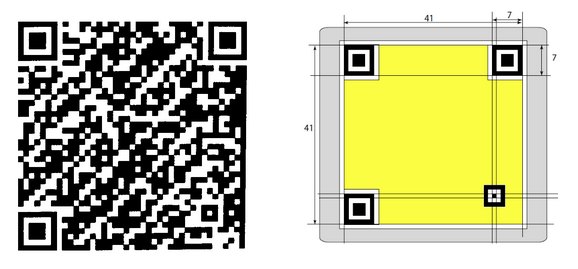
\includegraphics[width=0.9\linewidth]{./img/qr1.png}
   \captionof{figure}{\label{fig:qr1}\emph{To the left: an example of a QR-code version 6. To the right is the dimensions of the QR-code.}}
\end{Figure}

\section{Method}
The implementation in this study is passive without any interaction during the execution. The input is an image, containing a QR-code and the output is a string of text. The method for finding and extracting QR-codes is divided into several steps. Each step is described in its own subsection. Something worth mentioning is that operations that require interpolation, such as resizing, rotating and perspective projection are all made on a grayscale version of the original image. All steps in the pipeline are illustrated in Fig.\ref{fig:pipeline}. 
\begin{Figure}
  \centering
    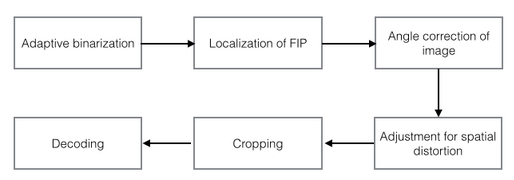
\includegraphics[width=1\linewidth]{./img/pipeline.png}
   \captionof{figure}{\label{fig:pipeline}\emph{All the steps in the pipeline for extracting QR-codes.}}
\end{Figure}

\subsection{Binarizing the Image}
In order to be able to manage images with a wide variation in brightness and contrast, an adaptive binarization function has been implemented. After the image has been converted to only contain grey scale values, the first step in the adaptive binarization function is to calculate an integral image from the original image.

An integral image, which is also known as a summed area table \cite{bradley} is a data structure where the sum of the pixel values in the original image is stored in the corresponding cell in the integral image. How this is done is illustrated in Fig.\ref{fig:integralimage}.
\begin{Figure}
  \centering
    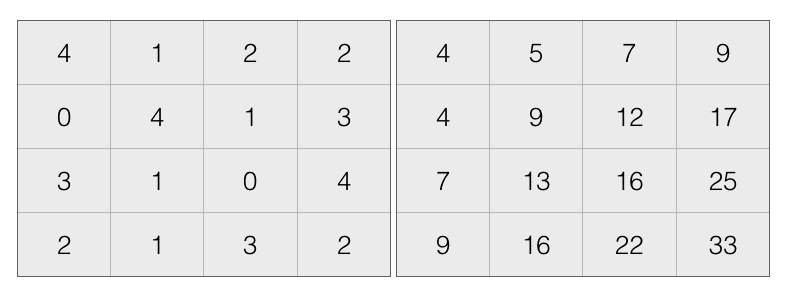
\includegraphics[width=1\linewidth]{./img/Integralimage.png}
   \captionof{figure}{\label{fig:integralimage}\emph{An intensity image to the left and its calculated integral image to the right.}}
\end{Figure}

When the integral image has been calculated a window of pixels is created. The size of this window is $1/8$ of the width of the image. This window is then passed over the image and the average of the values of the pixels in the integral image inside the window is calculated. If the current pixel is a certain percentage lower than the average of the window, the pixel in the original image is set to black. Otherwise the pixel is set to white. The percentage is set to 15\% \cite{bradley}. 

This method is only used in order to find the fiducial marks in the QR-code properly. It is not used in the last step when the decoding of the QR-code is done.

\subsection{Localizing the Fiducial Marks}
The so called fiducial marks are three shapes located in three of the corners of the QR-code. The fiducial marks have the shape of a square containing black and white pixels. The black and white segments of the square have the ratio 1:1:3:1:1 \cite{belussi} in the order black, white, black, white and finally black. By scanning the binarized version of the original image both horizontally and vertically segments of black and white pixels can be extracted. For each segment, the size of the segment and the pixel position where the segment ends are stored in a separate list. 
\begin{Figure}
  \centering
    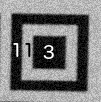
\includegraphics[width=0.7\linewidth]{./img/Fiducial.png}
   \captionof{figure}{\label{fig:fiducial}\emph{Image of a fiducial mark showing the ratios between black and white.}}
\end{Figure}

When all the segments in the image have been extracted, the list of segments is searched. First a black segment is looked up. Then the segments upwards, downwards, to the right and to the left are checked in order to determine if the ratio is fulfilled. When a match has been found, the corresponding pixel positions in an otherwise black image with the same size as the original image are coloured white. The result is a black image with small white fields where the algorithm has found a match. This enables labelling of the white fields in a later stage. 

If a match has been found or not is determined by the following code snippet. The snippet shows how it is done when scanning vertically.
\newpage
\begin{lstlisting}
findpattern = zeros(height, width);
percentage = 0.32;
%Check middle to adjacent
if abs(middleBlack-3*upWhite) <= percentage*middleBlack && abs(middleBlack-3*downWhite) <= percentage*middleBlack
	%Check the outer segments
	if abs(upWhite-upBlack) < percentage*upWhite && abs(downWhite-downBlack) < percentage*downWhite
		%Match is found, color the pixels in the black image white.
		%SegmentsY contains the pixel positions for the segments end.
		findpattern(segmentsY(i-2, 2):segmentsY(i+2, 2), segmentsY(i-2, 3):segmentsY(i+2, 3)) = 1;
	end
end
\end{lstlisting}
The result of this code snippet is shown in Fig.\ref{fig:findpattern}.
\begin{Figure}
  \centering
    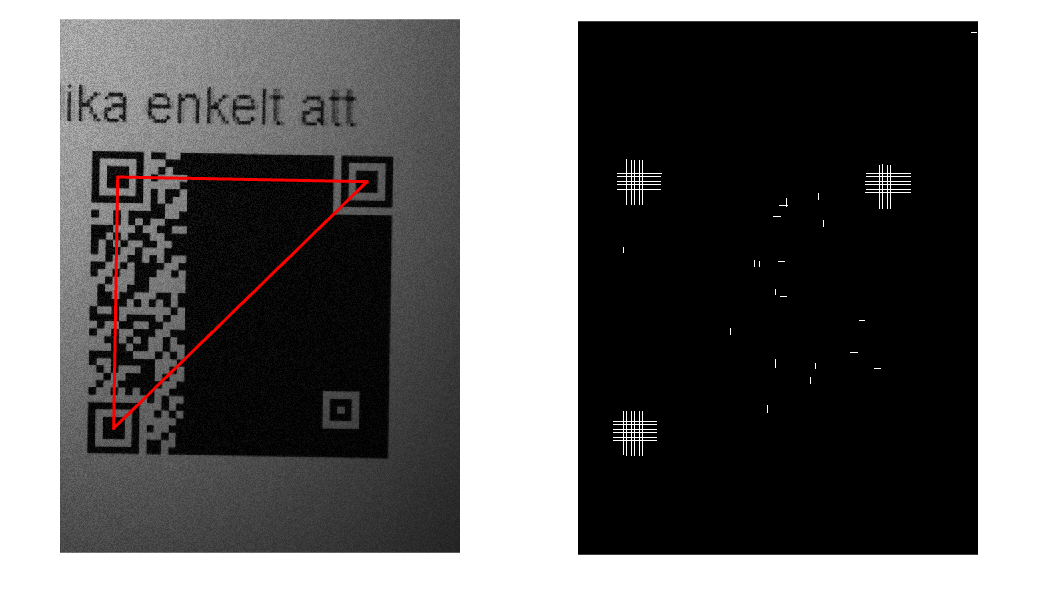
\includegraphics[width=1\linewidth]{./img/findpattern.png}
   \captionof{figure}{\label{fig:findpattern}\emph{Image of a fiducial mark showing the ratios between black and white.}}
\end{Figure}

When all the white fields in the otherwise black image have been labelled the center of these fields are determined. First a check is made determining if the white fields have a rectangular shape. Then the center of the rectangle is calculated. Sometimes false positives will cause the labelled field to not form a rectangular shape. In such case, the median coordinates of the field are chosen as center point. To make sure the center point is really in the center of the fiducial mark the pixels in the center of the fiducial mark are counted and the center point is moved to the exact center. 

\subsection{Rotation}
When the fiducial marks are detected that means that the QR-code is found in the image, but in order to decode the QR-code it needs to be straightened. The first step in the straightening process is to rotate the QR-code so that has the right orientation. Since the centers of all fiducial marks are now known, they can be used for rotation. In this implementation the two fiducial marks at the top are used. By subtracting one of the fiducial marks at the top from the other the vector between them will be achieved. By normalizing this vector and applying the dot product between it and the x-axis the angle between them can be calculated. This is illustrated in the equation Eq.\ref{eq:angle}.
\begin{equation}\label{eq:angle}
	\alpha = cos^{-1}(\hat{v} \cdot \hat{x})
\end{equation}
Where $\alpha$ is the achieved angle, $\hat{v}$ is the normalized vector between the fiducial marks and $\hat{x}$ is the x-axis. After the angle has been calculated a check is made whether the vector $\hat{v}$ has a negative x component. If that is the case the resulting angle $\alpha$ will be $\alpha=\alpha-\pi$. The image in Fig.\ref{fig:rotated} shows an image before and after rotation. 
\begin{Figure}
  \centering
    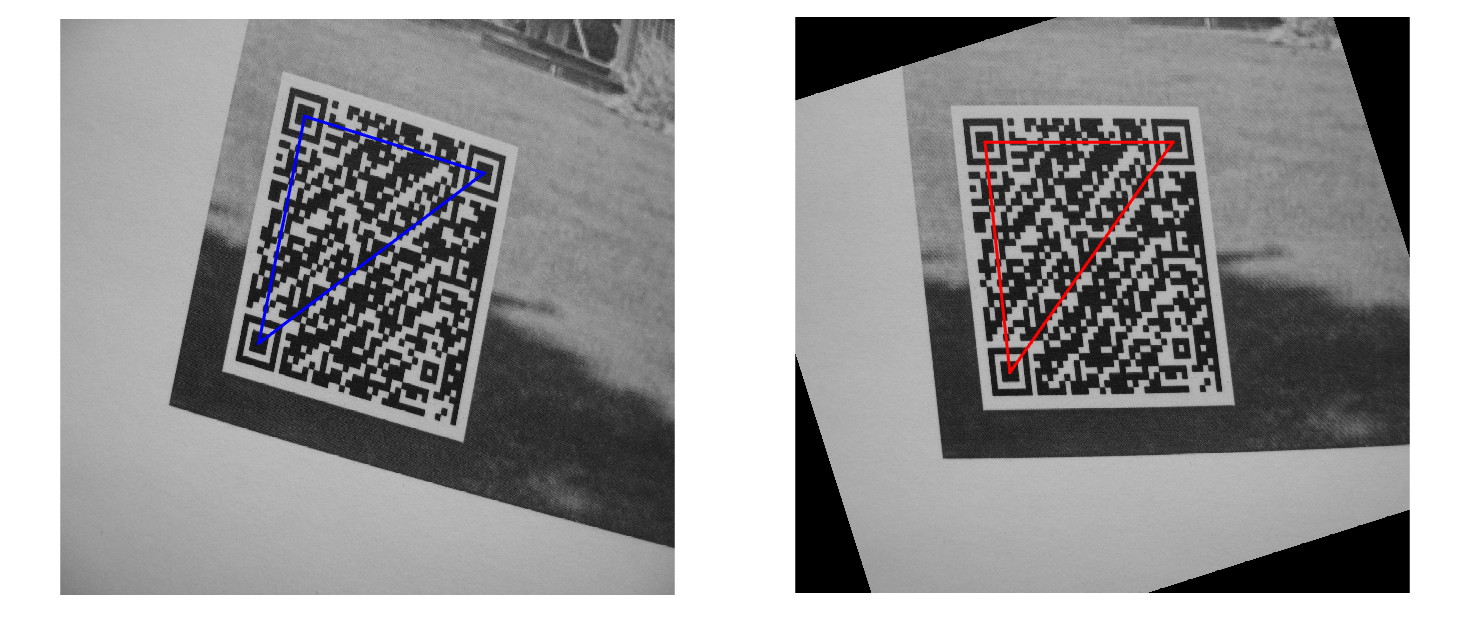
\includegraphics[width=1\linewidth]{./img/rotated.png}
   \captionof{figure}{\label{fig:rotated}\emph{Before rotation on the left, and after rotation on the right.}}
\end{Figure}

\subsection{Adjustment for Perspective Distortion}
Even though the QR-code is now rotated properly, it may still have spatial distortion that could possibly make the QR-code unreadable. The most common spatial distortion among the images in the training set given for this project is perspective distortion. To account for this, projective transformation was used. In projective transformation lines are mapped to other lines, in this implementation the corners of the QR-code together with the center point of the alignment pattern is used as tie points to perform the projective transformation.

\subsubsection{Corner Detection}
The projective transformation needs a minimum of two $4\times2$ matrices containing points from the image as input. The two matrices must match in size. One of the two matrices will be called \textit{fixed points} and the other one will be called \textit{moving points}.

The moving points - matrix should contain points in the image that are to be moved or mapped to new points. In this implementation the corners of the QR-code have been used. First, the corners where there are fiducial marks are found. This is done by first moving the center point of the fiducial mark by a factor of $7/6$ of the number of pixels in the black pixels in the center of the fiducial mark in either negative or positive x and y direction, depending on the corner. This will return a good estimate for where the corner should be. However, this estimate may not always be good enough depending on the amplitude of the spatial distortion. To make sure an even better corner point is achieved, a small area around the corner is extracted from the image. This small area is then used to more precisely determine where the corner is. 

The fourth corner in the lower right edge of the QR-code is found in a different way. In most versions QR-codes, or at least the ones used for this study, there is a so called alignment pattern in the lower right area of the QR-code. The alignment pattern consists of white and black pixels with the ratio 1:1:1 in all directions. Searching for this ratio over the whole image would generate too many false positives, making it difficult to determine where the alignment pattern really is. However, it can be found using the normalized 2D cross correlation. 

In order to use the normalized 2D cross correlation a template has to be created. The template is created to look like the alignment pattern, and is calculated the following way. As mentioned earlier, the black pixels in the center portion of the fiducial mark have been counted, which means the size of the center portion is known. By dividing the size of the center portion by 3, the approximated size of one bit in the QR-code is achieved. This can now be used to determine the size of the template. The size of the template should be 5 times as big as the size of one bit in the QR-code. Then the template is filled with black and white pixels in the order white, black and white. 

When the template has been created it is used to scan only lower right quarter of the QR-code. The normalized 2D cross correlation function is built in to Matlab and is called \textit{normxcorr2} \cite{normxcorr}. This function will return a correlation matrix with values spanning from -1 to 1. 

The normalized cross correlation between the template and the image is calculated using Eq.\ref{eq:correlation}.
\begin{equation}\label{eq:correlation}
	\gamma(u,v)=\frac{\sum_{x,y} [f(x,y)-\bar{f_{u,v}}]][t(x-u,y-v)-\bar{t}]}{\left \{ \sum_{x,y}[f(x,y)-\bar{f_{u,v}}]^2\sum_{x,y}[t(x-u,y-v)-\bar{t}]^2   \right \}^{0.5}}
\end{equation}
Where $\bar{t}$ is the mean value of the template, $\bar{f}_{u,v}$ is the mean value of the image currently under the template \cite{lewisfast}. 

By extracting the largest value from the correlation matrix the coordinates for the alignment pattern are achieved. These coordinates together with the coordinates for the other corners are then saved in the moving points - matrix. 
\begin{Figure}
  \centering
    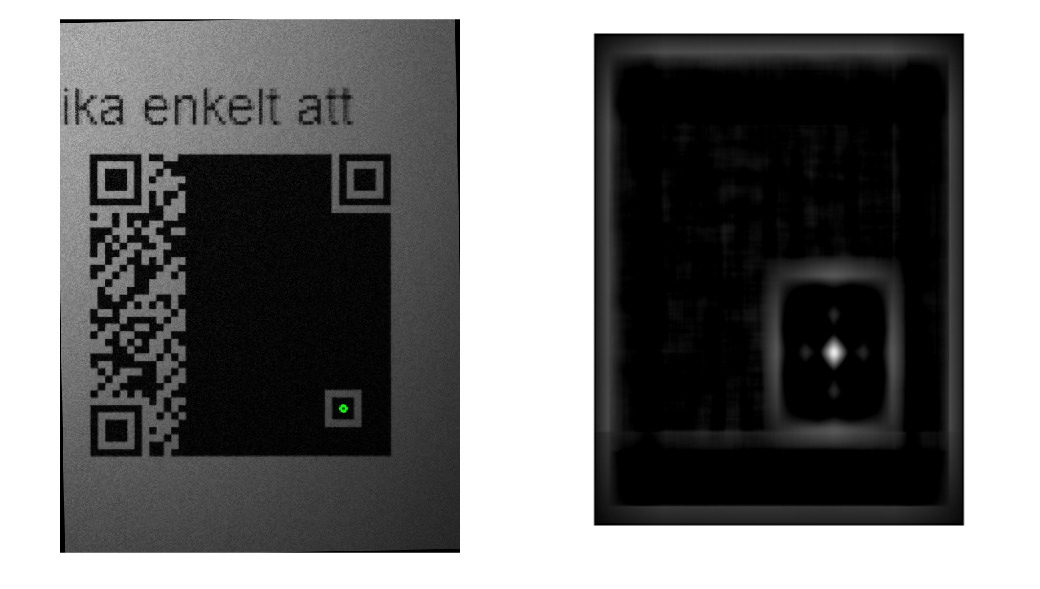
\includegraphics[width=1\linewidth]{./img/correlation.png}
   \captionof{figure}{\label{fig:correlated}\emph{To the right: the correlation matrix visualized. To the left: The center of the alignment pattern marked with green.}}
\end{Figure}

The fixed points - matrix contains the points we want to move the moving points to. These are our desired, straight points. These points are calculated by using the same size for one bit in the QR-code calculated in the previous step. The estimated height and width are achieved by multiplying the size on one bit by 41, since it is known that the QR-code size is 41x41 bits. Now the coordinates of three desired corners are determined. By calculating three corners, the fourth corner also achieved no extra calculations needed. The fourth corner can be used to calculate where the alignment pattern should be in the straightened up image. The alignment pattern should be seven bits from the fourth corner in both x and y direction. When all these corners have been determined they are passed in to the projection function. 

\subsubsection{Projective Transformation}
The most common distortion that could be fixed with this transform is the perspective distortion where the image was taken from a view with some perspective angle to the QR-code. The established four corner points together fix the calculated fixed points a transformation matrix could be calculated according to Eq.\ref{eq:tmatrix}.
\begin{equation}\label{eq:tmatrix}
	Tx=x{}'
\end{equation}
\begin{equation}\label{eq:tmatrix2}
	\begin{pmatrix}
		A & B & C\\ D & E & F \\ G & H  & 1 
	\end{pmatrix}\cdot 
	\begin{pmatrix}
		x_1 & x_2  & x_3  & x_4 \\ 
		y_1 & y_2 & y_3 & y_4 \\ 
		1 & 1 & 1 & 1 
	\end{pmatrix} =
	\begin{pmatrix}
		{x_1}' & {x_2}'  & {x_3}'  & {x_4}' \\ 
		{y_1}' & {y_2}' & {y_3}' & {y_4}' \\ 
		1 & 1 & 1 & 1 
	\end{pmatrix}
\end{equation}
\begin{equation}\label{eq:tmatrix3}
	T=x'x^{-1}
\end{equation}
A linear equation represented by a transformation matrix applied on the fixed points that is equal to the corner points can be used to extract the transformation matrix in Eq.\ref{eq:tmatrix} and Eq.\ref{eq:tmatrix3} \cite{projective}.
Since we have four points with two coordinates there will be total eight linear equations to solve.

In Eq.\ref{eq:tmatrix3} the inverse of the fixed points multiplied with the corner points will give the transformation matrix. This inverse could be solved by using Moore-Penrose pseudo inverse \cite{penrose}. The inverse of the transformation matrix will have to be calculated since the transformation matrix corresponds to the transformation from the fixed points to the distorted corner points which means that the inverse is the desired transformation matrix.

In matlab the function called \textit{fitgeotrans} \cite{fitgeotrans} was used and it basically returns a transformation matrix and uses a built in solver to linear equations which uses a least square solution similar to the Moore-Penrose pseudo inverse \cite{mldivide}. This transformation matrix, together with the original image are sent in to the function \textit{imwarp} \cite{imwarp}. This function applies the transformation matrix to the image and interpolates new sample values in the image with nearest neighbour interpolation. 
\begin{Figure}
  \centering
    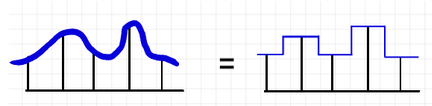
\includegraphics[width=1\linewidth]{./img/nearestnei.png}
   \captionof{figure}{\label{fig:nearest}\emph{Neareast neighbour interpolation takes the value of the closest sampled point.}}
\end{Figure}
The projective transformation together with the rotation is the geometric restoration in this implementation. The result before and after the transformation is shown in Fig.\ref{fig:perspective}.

\begin{Figure}
  \centering
    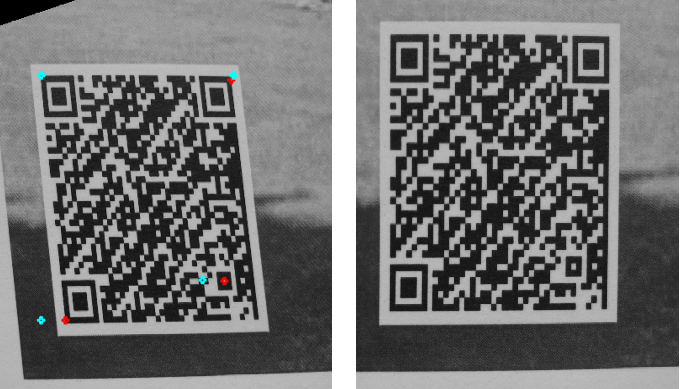
\includegraphics[width=1\linewidth]{./img/perspectivefinal.png}
   \captionof{figure}{\label{fig:perspective}\emph{To the left: Red dots represent moving points. Cyan dots represent fixed points. The point in the upper left corner is the same for both fixed and moving points. To the right is the image after projective transformation.}}
\end{Figure}

\subsection{Cropping}
When the image has been corrected for perspective distortion, the QR-code is cropped from the image. Since the image now should be rated and transformed properly, this step can be made without the risk of losing any information. The rectangle which spans the area used for cropping is the same rectangle use in the fixed points - matrix mentioned in the previous section. This is possible since the image is warped and mapped to match the fixed points. When the QR-code has been cropped from the image, the QR-code is resized so that it becomes a square image. 

\subsection{Decoding the QR-code}
At this stage a perfect binary image of the QR code without the silent area in the best situation is the input to this function. This is where the information in the QR-code is translated into bits and then to characters using the ASCII table. 

First the dimension of the images gets divided into 41x41 since the version 6 QR-codes has these dimensions. The fiducial marks and the alignment pattern gets ignored and all bits in sequence of 8 bits(1 byte) gets translated into a characters and saved in a char array. The image is scanned vertically and when all information in the QR code has been decoded the char array gets transformed into a string and returned as the final result.
\begin{Figure}
  \centering
    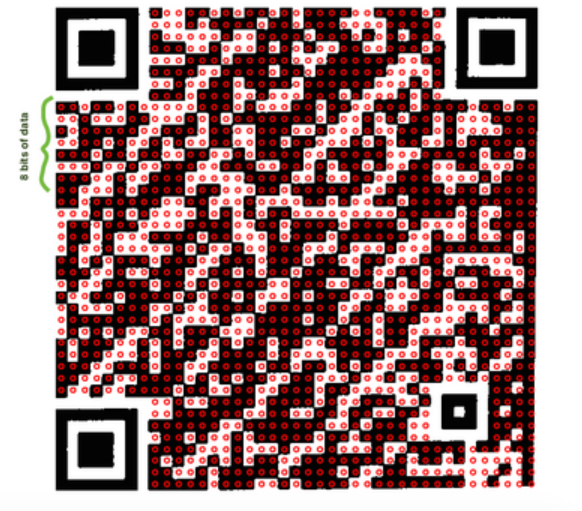
\includegraphics[width=1\linewidth]{./img/decoding.png}
   \captionof{figure}{\label{fig:decoding}\emph{The red dots represent the position where each bit get their value from.}}
\end{Figure}

\section{Result}
The implementation has been tested on 54 images that include three different images in different rotations, distortions and resolution. In the test all images are decoded correctly but returns an error for one image where a capital A is return instead of a lower case a. The reason for this error is unknown.
\begin{table}
    \begin{tabular}{|l|l|l|}
    \hline
    \textbf{Name of folder}          & \textbf{Images where decoding fails} & \textbf{Successful decoding} \\ \hline
    Images\_Training\_1     & None                        & 100 \% (24/24)      \\ \hline
    Images\_Training\_2     & None                        & 100 \% (6/6)        \\ \hline
    Images\_Training\_3     & Hus\_2e.png                 & 83,3 \% (5/6)       \\ \hline
    Images\_Training\_4     & None                        & 100 \% (6/6)        \\ \hline
    Images\_Training\_5     & None                        & 100 \% (8/8)        \\ \hline
    Images\_Training\_Illum & None                        & 100 \% (4/4)        \\ \hline
    \textbf{Total}                   & \textbf{Hus\_2e.png }                & \textbf{98,1 \% (53/54)}     \\ \hline
    \end{tabular}
    \caption{\label{tab:result}Result of the training set.}
\end{table}

\section{Conclusion and Discussion}
\textit{A summary of the performed work together with a discussion of why the different approaches in this project are good or bad and of improvements that could be made.} 

The program works for the majority of the images tested with an fairly good performance. 
It can extract QR-codes and decode them in images with quite the amount of distortion and rotation. Given the time spent on this project we are satisfied with the result, but there are many things that could be improved in future work.

\subsection{Performance}
Matlab is a powerful and fast tool to use when using matrix operations. In a problem like this, where a lot of searching in images has to be made, Matlab is not very fast since traditional loops are not really optimized. There is one place in the implementation where the whole image to be scanned. This is the step where the fiducial marks are found. This step is by far the slowest part of the implementation, even though optimizations have been made such as only scanning every fourth pixel, preallocating space and using the Matlab function \textit{bwconncomp} which returns all connected white pixels. The function \textit{bwconncomp} was used instead of counting pixels in the initial step of the implementation. 

\subsection{Corner detection}
The corner detection used in this implementation is sensitive for noise since the algorithm only compares two points in the close neighbourhood of the corner. If there is noise present, there is a risk that the algorithm returns a bad corner. The corners will never be perfectly detected but close enough to achieve an image where it is possible to decode the QR-code. But the corners will lose precision the more geometric distortion there is and at some point the corner will be too inaccurate to use.

Possible solutions could be to implement an well known corner detection like Harris-Stephens algorithm to find a more accurate corners and to find the corner in cases where the geometric and distortion is very intense.

\subsection{Transformations}
The most common distortion in the test images seems to be perspective distortion. Therefore this is the only kind of geometric distortion accounted for. If other geometric distortions like Barrel and Pincushion distortion would be present, the correction may be wrong since there is only four tie points used for extracting a transformation matrix and that is too few to restore this kind of distortion. 

\subsection{Special cases}
As mentioned the implementation works for images with quite much distortion and rotation but if the distortion and rotation would be more extreme, it would probably not work. If the rotation is very big like 90 degrees or more the program would fail since the fiducial marks and alignment patterns would be at the wrong positions and no check is done for this at the moment but could be a good improvement to implement. The algorithm would also fail if the QR-code is flipped.

Also if an image has none or more than one QR-code the implementation would probably fail since it is limited to only be able to find one QR-code. If no QR-code is detected, a future version could possibly give some kind of error message back to the user. 

The case where the image have much camera shake distortion[Ref] is also not considered and could be a possible improvement to add to the pipeline. 
 
% optional bibliography
%\begin{thebibliography}{99}

%\end{thebibliography}

\bibliography{aBoBreport.bib}{}
\bibliographystyle{plain}
 
\end{document}